\documentclass[fleqn]{article}

\usepackage{mydefs}
\usepackage{notes}
\usepackage{url}
\usepackage{graphicx}

\begin{document}
\lecture{Alex Clemmer u0458675}{HW1: K-Nearest Neighbors and Decision Trees}{Due: September 20}


\section{Written Exercises}

\bee

\i The $K$-nearest neighbors method makes the prediction $y$ for a new
test point $x$ by either taking a majority vote (for classification) 
, or by doing averaging (for regression) using the labels of its
$K$ most similar training examples. Assume $\mathcal{N}$  to be the 
set of these examples. For the classification setting, finding the majority 
amounts to finding the most frequent labels in the set $\mathcal{N}$. For 
binary classification, (assuming $y_i \in \{-1,+1\}$) this is simply 
equivalent to $y = \sign(\sum_{j \in \mathcal{N}} y_j$). For the regression 
setting (assuming $y_i \in \mathbb{R}$), the averaging rule is simply 
$y = \frac{1}{K}\sum_{j \in \mathcal{N}} y_j$.  However, both these rules 
assume that we trust each of the nearest neighbors equally which may not be 
what we want. For example, assuming $K = 3$, we may have a case that a test 
example has one \textit{very very similar} training example with label -1 
and two \textit{relatively much less similar} training examples with label +1. 
In such a case, although it might make more sense to assign label -1 to 
this test example but the standard $K$-nearest neighbor algorithm would say +1.
A way to address this issue would be to assign a weight $w_i$ to each 
training example's label $y_i$. $w_i$ basically is a measure of how similar
$x_i$ is to the test example. We can then \textit{somehow} use these weights 
in making the prediction for the test point. How would you compute these weights, 
and how would you use these for $k$NN based binary classification and regression 
(write the rules in form of equations)?

\begin{solution}
One simple solution is to simply apply to each neighbor a weight $w_i = \frac{1}{d}$, with $d$ being the (typically Euclidean) distance between the neighbor and test point $x$. If we have a weight function $W$ that outputs such weights, then obtaining the weighted votes is generally pretty straightforward in the case of \textbf{regression}:

\begin{equation}
y = \sum_{j = 1}^k W(x_0, x_1) y_j
\end{equation}

The case of \textbf{classification} can be done simply by applying a number of votes proportionate to some weight $w_i$. One obvious solution is to invert the weight (which remember is typically $\frac{1}{d}$) to get $d$ votes for that particular label:

\begin{equation}
y = \sum_{j = 1}^k W(x_0, x_1)^{-1} y_j
\end{equation}

\end{solution}

An alternative to the $K$-nearest neighbors is called the $\epsilon$-ball
method. Instead of finding the $K$ nearest neighbors in the training 
data, you construct a ball with radius $\epsilon$ around the test point
and take the majority vote (for classification) or do averaging (for regression)
of all training examples lying inside this ball. The parameter $\epsilon$ (just 
like $K$) is user specified. Do you think this alternative fixes the 
above-mentioned problem of the $K$-nearest neighbors? If yes, do you think this 
is better than the weighting scheme of $K$-nearest neighbors we talked about 
above? If yes, why? If no, why not?

\begin{solution}
As George Box says, all models are wrong, but some are useful. The $\epsilon$-ball model does address the problem that $k$NN in the general case can and does treat poor examples and good examples prettty much the same; and indeed, if the radius of the $\epsilon$-ball is chosen well, then this issue is more or less solved. There is one major advantage, though, with the weighted $k$NN scheme, and that is that it works with pretty much no configuration. In fact, at least one formulation (Shepard '68) uses arbitrarily large $k$ and gives the most important queries the proper weight, similar to the outline above. This is a feature that it is really hard to compensate for with $\epsilon$-ball.
\end{solution}


\i For real-valued features, the ``standard'' notion of distance 
that we talked about in the class is the Euclidean distance. 
In particular, we measure the distance between two vectors $\vec x$ 
and $\vec y$ by the \emph{Euclidean norm} of the vector $\vec z$ 
defined by $\vec z = \vec x - \vec y$.  The Euclidean norm is, of 
course, defined by $\norm{\vec z} = (\sum_d z_d^2)^{1/2}$.  There 
are other norms that one can define.  In fact,
there's a whole class of them, called the $\ell_p$ norms.  The
$\ell_p$ norm, $\norm{\cdot}_p$ is defined below (for $p>0$):
\begin{equation*}
\norm{\vec z}_p = \left(\sum_d \ab{z_d}^p\right)^{\frac 1 p}
\end{equation*}
Here, $\ab{a}$ means the absolute value of $a$.  It's easy to see that
the Euclidean norm is exactly the $\ell_2$ norm.  The $\ell_1$ norm is
just $\norm{\vec z}_1 = \sum_d \ab{z_d}$.  This is also known as the
\textbf{Manhattan norm} because it measures distances by the number of
``blocks'' that one would have to walk to get between two points, when
roads only run along axes (think of the roads in the Salt Lake City :)).

Consider the case of using a $k$NN classifier, but with the $\ell_1$
norm to measure distances rather than the $\ell_2$ (Euclidean) norm.
Draw in two dimensions (i.e., each example has only two features) 
a simple case of a binary classification problem for which the 
$\ell_1$ classifier would return a different class for a test point 
than an $\ell_2$ classifier.  In particular, draw $\geq 1$ training 
points (one for each class) and a test point that would be classified 
differently according to the two distance metrics.

\begin{solution}
We can trivially generate Cartesian coordinates that the heuristics disagree on. Imagine that our query is \textbf{(0,0)} and our trained points are \textbf{\{(10,10) (18, 1)\}}, each with a \textbf{different label}. In the case of \textbf{Manhattan} we pick the second:

\begin{equation}
\norm{\vec z}_1 = \sum_d \ab{\{10, 10\}} = 20
\end{equation}

\begin{equation}
\norm{\vec z}_1 = \sum_d \ab{\{18, 1\}} = 19
\end{equation}

Yet in the case of the \textbf{Euclidean}, we pick the first:

\begin{equation}
\norm{\vec z}_2 = \left(\sum_d \ab{\{10, 10\}}^2\right)^{\frac 1 2} \approx 14.142
\end{equation}

\begin{equation}
\norm{\vec z}_2 = \left(\sum_d \ab{\{18, 1\}}^2\right)^{\frac 1 2} \approx 18.02
\end{equation}

\end{solution}

\begin{solution}
We can similarly come up with another set of points using the same pattern. Let's again imagine that the test query is \textbf{(0,0)}, and the trained data is \textbf{\{(25, 4) (21, 10)\}}, each with a different classification perscription. For the \textbf{Manhattan}, we pick the first point:

\begin{equation}
\norm{\vec z}_1 = \sum_d \ab{\{25, 4\}} = 29
\end{equation}

\begin{equation}
\norm{\vec z}_1 = \sum_d \ab{\{21, 10\}} = 31
\end{equation}

And for the \textbf{Euclidean}, we pick the second:

\begin{equation}
\norm{\vec z}_2 = \left(\sum_d \ab{\{25, 4\}}^2\right)^{\frac 1 2} \approx 25.318
\end{equation}

\begin{equation}
\norm{\vec z}_2 = \left(\sum_d \ab{\{21, 10\}}^2\right)^{\frac 1 2} \approx 23.259
\end{equation}

\end{solution}

What properties of a data set do you imagine would influence whether
the $\ell_1$ distance would work better or worse than the $\ell_2$
distance?

\begin{solution}
$\ell_1$ is first of all likely to be more effective for problems that can be expressed as a grid, and in which actors can only move under stricture of that grid (\textit{e.g.}, a car on a street). You could, for example, probably express things like Levenshtein distance and string diffs (\textit{i.e.}, the number of discrete transformations it takes to change one string into another) in terms of $\ell_1$. But wherever this sort of characterization is not the case, this probably becomes a less good mechanism, and generally speaking, the more free the movement is, the better $\ell_2$ will be in comparison.
\end{solution}

\i (\textit{6350 only}) An important notion for a classifier is that 
of consistency. Roughly, a classification algorithm is consistent if, 
whenever it has access to infinite amounts of training data, its error rate
approaches the optimal error rate (aka, Bayes optimal). Consider the 
noise-free setting. Here, the Bayes optimal error rate is zero. Is the 
one-nearest-neighbor algorithm consistent in this setting?

\i Assume that we are learning the ID3 decision tree to do classification, and
 at one stage, there are nine training examples remaining, five positive and 
four negative. We have the choice of splitting on two binary features A or B. 
When A is true, there are two positive and three negative examples; when A is 
false, there are three positive and one negative examples. On the other hand, 
when B is true there is three positive and three negative examples; when B is 
false there are two positive and one negative examples. Which feature will ID3 
choose to split on? Show the information gain calculations.

\begin{solution}
The information gain for the various choices break down as so:

\begin{eqnarray*}
S = [5+, 4-] \Rightarrow H(S) = -(5/9) \mbox{log}_2 (5/9) - (4/9) \mbox{log}_2 (4/9) & \approx & 0.99108 \\[0.1in]
S_{Atrue} = [2+, 3-] \Rightarrow H(S_{Atrue}) = -(2/5) \mbox{log}_2 (2/5) - (3/5) \mbox{log}_2 (3/5) & \approx & 0.97095 \\
S_{Afalse} = [3+, 1-] \Rightarrow H(S_{Afalse}) = -(3/4) \mbox{log}_2 (3/4) - (1/4) \mbox{log}_2 (1/4) & \approx & 0.81128 \\[0.1in]
S_{Btrue} = [3+, 3-] \Rightarrow H(S_{Btrue}) = -(3/6) \mbox{log}_2 (3/6) - (3/6) \mbox{log}_2 (3/6) & = & 1 \\
S_{Bfalse} = [2+, 1-] \Rightarrow H(S_{Bfalse}) = -(2/3) \mbox{log}_2 (2/3) - (1/3) \mbox{log}_2 (1/3) & \approx & 0.9183
\end{eqnarray*}

Pluggin these in is fairly straightforward:

\begin{eqnarray*}
IG(S, A) = 0.99108 - \frac{5}{9} \cdot 0.97095 - \frac{4}{9} \cdot 0.81128 & \approx & 0.091094 \\[0.05in]
IG(S, B) = 0.99108 - \frac{6}{9} \cdot 1 - \frac{3}{9} \cdot 0.9183 & \approx & 0.018313 \\
\end{eqnarray*}

Clearly we will split on A.

\end{solution}

\i Recall that under any subtree of the decision tree, a feature that has already 
been tested before need not be tested. Assume that there are $F$ binary-valued 
features in the data. How many information gain calculations would be needed to 
construct the full decision tree (i.e., assuming no pruning)?

\begin{solution}
We begin building the tree by finding the binary-valued feature with the highest information gain at root. This process gives us leaves. We then recursively repeat this for each of those leaves until stopping criteria are satisfied for some branch (\textit{i.e.}, when all remaining samples are the same, when there are no samples left, or you run out of features). Since we have to compute a different information gain every time we add a feature to the tree, we must perform $O(n!)$ such calculations.
\end{solution}

\i (\textit{6350 only}) Intuitively, the information gain criteria prefers to use 
features that split a node such that the child nodes are as \textit{homogeneous} 
as possible. For the classification setting, it means that the split would ideally 
like each of the child nodes to have one of the labels dominate the others (i.e., 
-1 labels dominating +1 labels, or vice-versa). Using the similar intuition, what 
would be a good criteria (other than information gain) for splitting if we were 
doing regression instead of classification (so the labels are real-valued numbers 
instead of discrete variables like +1/-1)?

\ene

\section{Programming Exercises}

\bee

\i Your task is to implement the prediction phase of $K$-NN for classification. 
There is shell code for this in \texttt{KNN.m}. Your job is to implement the 
subroutine called \texttt{KNNpredict}. This takes as input the training data 
points (with labels), a value for $K$ and a single test point. Its output 
should be the most frequent label among the $K$ closest points in the training 
data to the test point. Your implementation should be robust to handle the 
multiclass classification.

Apply this classifier to the provided dataset (it's a binary classification dataset). 
The dataset has three parts: training, development, and test set. In each file, each
row represents an example. The first value in each row is the label and the rest of the 
values are the features. To load this data in MATLAB, simply do \texttt{data = 
load('hw-train');}. To get the labels Y, do \texttt{Y = data(:,1);} and to get the 
features do \texttt{X = data(:,2:end);}. Likewise for the development and the test data.

For your implemented classifier, allow $K$ to range over all \textit{odd integers} 
in [1; 20] and plot validation, and test error as a function of $K$. At which 
value of $K$ is the development error minimized? At which value of $K$ is the test 
error minimized?

\begin{solution}
For me, the error was minimized for development at $k = 17$ and for test at $k = 7$. Please see the code I wrote and run the tests for yourself if you see fit.

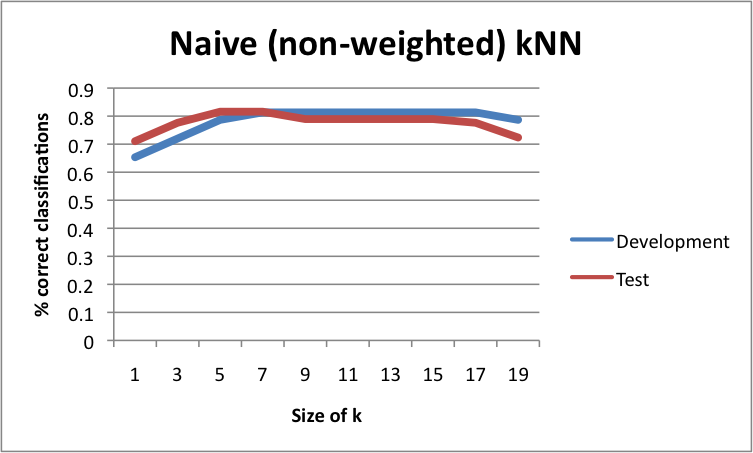
\includegraphics[scale=0.8]{Naive.png}
\end{solution}

\i Re-implement the \texttt{KNNpredict} routine so that it allows the weighting strategy 
we discussed in the written excercise (1) for the binary classifications setting
(where the \textit{unweighted} majority rule can be expressed as $y = \sign(\sum_{j 
\in \mathcal{N}} y_j$). Test your implementation on the provided dataset from part-1. 
Again allow $K$ to range over all \textit{odd integers} in [1; 20] and plot development, 
and test error as a function of $K$. At which value of $K$ is the development error 
minimized? At which value of $K$ is the test error minimized?

\begin{solution}
This straight up did not do as well as I thought it would. This is probably my fault, though I didn't quite have enough time to develop it into what it could/should have been. Anyway, I've included graphs that both look at weigted $k$NN alone and compare it to naive $k$NN, and you'll see that they actually do comparably, so I doubt that I messed up horribly.

For the dev data, $k = 19$ was my best, while for testing it was $k = 17$.
\end{solution}

\begin{solution}
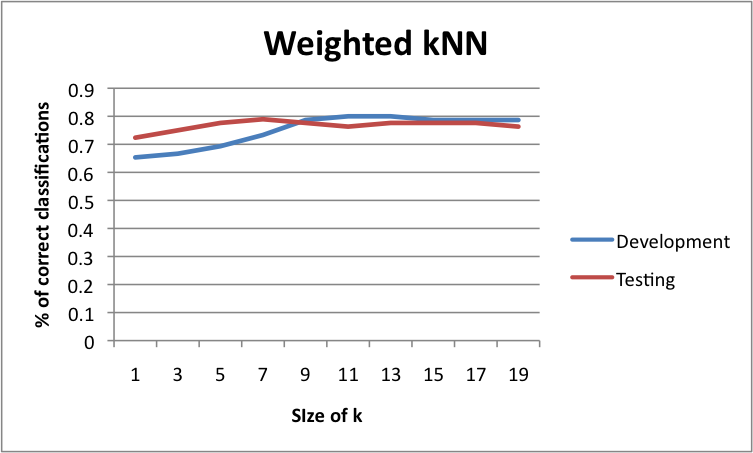
\includegraphics[scale=0.8]{Weighted.png}
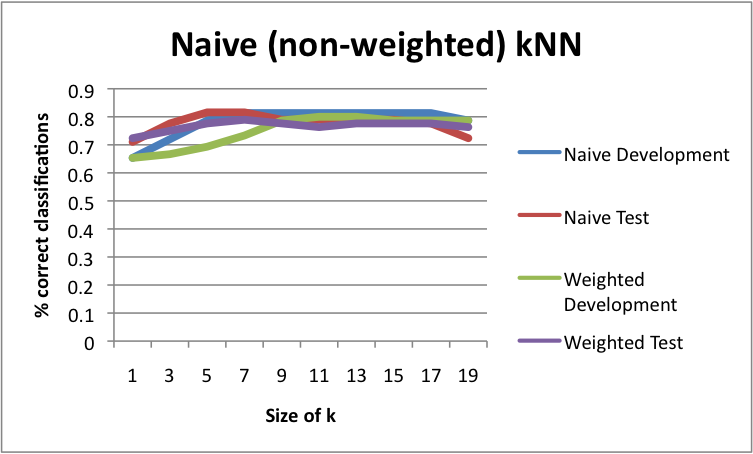
\includegraphics[scale=0.8]{Comparison.png}
\end{solution}

\ene

\end{document}
